\documentclass[aps, prb]{revtex4-1}
\usepackage{graphicx}
\usepackage{subfigure}
\usepackage{amsmath}
\usepackage[bookmarks, hyperindex, colorlinks=true,
            linkcolor=red,
            urlcolor=blue, citecolor=blue]{hyperref}

\usepackage{bm}
\graphicspath{{./figures/}}
\usepackage[usenames,dvipsnames,svgnames,table]{xcolor}

\renewcommand{\vec}[1]{\bm{#1}}
\newcommand{\subfigimg}[3][,]{%
  \setbox1=\hbox{\includegraphics[#1]{#3}}% Store image in box
  \leavevmode\rlap{\usebox1}% Print image
  \rlap{\hspace*{47.5pt}\vspace*{45pt}\raisebox{\dimexpr\ht1-2\baselineskip}{#2}}% Print label
  \phantom{\usebox1}
}

\begin{document}
\title{Downfolding: effective model construction from first principles simulation}
\author{Huihuo Zheng}
\email{huihuo.zheng@anl.gov}
\affiliation{
Argonne Leadership Computing Facility, Argonne National Laboratory, 9700 Cass Avenue, Lemont, 60439, Illinois, USA}
\date{\today}
\begin{abstract}
In this note, I will summarize the basic formalism of downfolding, with demonstration of several systems including molecules and solids. The results are based on Chapter 4 and Chapter 6 of my PhD dissertation \cite{Zheng2016}. 
\end{abstract}

\maketitle
\newcommand{\newt}[1]{{#1}}
\section{Introduction}
Physicists usually like to have an intuitive understanding of physical phenomena using simplified models. These models are expected to capture the most relevant physical degrees of freedom related to the observed phenomena. For example, at high temperature and low density when quantum effect is not significant, the ideal gas model can successfully capture the statistical properties of $10^{23}$ H$_{2}$ molecules in a box, without any detailed knowledge of the fundamental constituent of H$_{2}$. This approach is valid when we are interested in phenomena at certain energy scale (or length scale), while the degrees of freedom at other length scales which are not dynamically excited simply renormalize the dynamics of the low energy degrees of freedom. 

This concept/principle has been widely employed in condensed matter physics. For example, in the past decades, there are a lot of studies on describing complex systems (high Tc Cuprate and many other transition metal oxides) using models such as Hubbard model \cite{Yanagisawa2008}, t-J model \cite{Sorella2002}, etc. However, very few studies have addressed the effectiveness of those models in describing the real complex systems. In complex systems such as high Tc cuprates, it is unclear to what extent can these models describe the reality \cite{Anderson2013}. Generally, in strongly correlated systems, the macroscopic phenomena are strongly dependent on material-specific properties, motivating the need to determine the effective Hamiltonians that can capture all necessary details. 

On the other hand, the reliable simulation of systems for which the large-scale physics is not well-approximated by a non-interacting model, is a major challenge in physics, chemistry, and materials science. These systems appear to require a multi-scale approach in which the effective interactions between electrons at a small distance scale are determined, which then leads to a coarse-grained description of emergent correlated physics. This reduction of the Hilbert space is often known as ``downfolding".

A schematic of ``downfolding'' is depicted in Fig.~\ref{fig:effham}. The full Hamiltonian $H$ is defined in the space of active (partially occupied), core (mostly occupied) and virtual (mostly unoccupied) orbitals. These orbitals have been arranged according to their energy (E) in the figure. 
The objective is to map the physics of the original system to that of the effective one, defined only in the active space, with Hamiltonian $\tilde{H}$. Once an effective model Hamiltonian in the reduced Hilbert space  is obtained,  it can be used to perform a calculation on a larger system using techniques designed for 
lattice models~\cite{White1992,tps_nishino,Vidal_MERA,TPS_review,Changlani_CPS,
Neuscamman_CPS,mezzacapo,Marti,DMET_2012,Chen_DMET,Sandvik_loops,Blankenbecler,Alavi_FCIQMC,SQMC}. This multi-step modeling procedure is needed since the {\it ab initio} 
calculations for a given system size are, in general, 
computationally more expensive than the equivalent lattice calculations. 
Large sizes are crucial to study finite size effects, and in turn 
theoretically establish the presence of a phase. 
In addition, excited states and dynamical correlation functions have traditionally 
been difficult in {\it ab initio} approaches, 
but have seen progress for lattice model methods~\cite{Jeckelmann2002, Daley_tDMRG, White_tDMRG}.
\begin{figure}[htpb]
\centering
\includegraphics[width=0.4\linewidth]{./downfolding_scheme.pdf}
\caption{\newt{Schematic for downfolding. The full Hamiltonian H is defined in the space of active (partially occupied), 
core (mostly occupied) and virtual (mostly unoccupied) orbitals. These orbitals 
have been arranged according to their energy (E) in the figure. The objective is to map the physics 
of the original system to that of the effective one, defined only in the active space, 
with Hamiltonian $\tilde{H}$.}}
\label{fig:effham} 
\end{figure}


One can loosely categorize downfolding techniques into two strategies.
The first strategy is based on performing {\it ab initio} calculations and 
then matching them state by state to the effective model. Alternately, 
some approaches employ a model for the 
screening of Coulomb interactions, for which the {\it ab initio} single particle wavefunctions provide the relevant inputs. 
Techniques that fall into this class include the constrained 
density functional theory~\cite{Pavirini,Dasgupta}, 
the constrained random phase approximation (cRPA)~\cite{Aryasetiawan}, 
fitting spin models to energies~\cite{Valenti_kagome,Spaldin}, 
and fitting reduced density matrices of quantum Monte Carlo (QMC) calculations to that of model Hamiltonian~\cite{Wagner2014}. The second class is based on L\"owdin downfolding~\cite{Freed,Zhou_Ceperley,Tenno} 
and canonical transformation theory~\cite{Glazek_Wilson,Wegner,White_CT,Yanai_CT,Watson_Chan}, 
which involves a sequence of unitary transformations on the 
bare Hamiltonian, chosen in a way that minimize the size of the matrix elements 
connecting the relevant low energy (valence) space to the high energy one.

Downfolding by fitting has the advantage that it 
is conceptually straightforward to perform, although it demands an 
{\it a priori} parameterization of the effective Hamiltonian. 
The methods have been applied to complex bulk systems~\cite{Imada1,Imada2,Arya1,Arya2,Scriven,Wehling2011}, but it 
is only recently that their 
accuracy is being rigorously checked~\cite{RPA_Troyer}. 
On the other hand, canonical transformations do not need 
such parameterizations and can discover the relevant terms in an automated way. 
However, their application to complex materials remains to be carried out 
and tested.


In this note, we demonstrate three downfolding methods that use data from {\it ab initio} QMC techniques to derive an effective coarse-grained Hamiltonian.
\begin{itemize}
\item [(1)] Eigenstate {\it ab initio} density matrix downfolding (E-AIDMD): we optimize model parameters to match the density matrix and energy spectrum of the model Hamiltonian to that of the {\it ab initio} system. In this method, we build a one to one correspondence between the states of the model Hamiltonian and that of the \textit{ab initio} Hamiltonian. To accomplish this, we need to solve both the model Hamiltonian and the \textit{ab initio} Hamiltonian. Generally, we need to find a cheaper way to solve model Hamiltonian such that we can efficiently solve it multiple times for different parameters in order to find the optimized set of parameters that can match the \textit{ab initio} system. 
\item [(2)] Non-eigenstate {\it ab initio} density matrix downfolding (NE-AIDMD): this is based on the fact that, once a model Hamiltonian is assumed, the energy expectation  of a certain state is directly related to the reduced density matrix on that state. Thus, each state imposes a constraint for the model parameters. We can choose several low lying states (not necessary to be the eigenstates of the system), and form a linear least fitting problem for the model parameters. Solving the linear least problem will determine the value of the parameters. Meanwhile, analyzing the residue of the fitting also give us a quantitative estimate of how good the model is.
\item [(3)] Non-eigenstate {\it ab initio} EKT (extended Koopmans' theorem) matrix downfolding (EKT-AIDMD): this is similar to the NE-AIDMD, except that now we use the EKT matrices $\mathcal{V}$ and $\mathcal{C}$ [see Eqs.~\eqref{eq:vijv} and \eqref{eq:vijc}] instead of energy. Compared with NE-AIDMD, we have much more information (all the matrix elements of $\mathcal{V}$ and $\mathcal{C}$) in EKT-AIDMD to impose constraints on the parameters, instead of just the energy expectation for a particular state. Through the quality of the linear least fit, one can also assess the quality of the low energy model in describing the low energy physics of the system. 
\end{itemize}

In the following section, we will first provide detailed formulation of the three downfolding methods. We will then use the three methods to study the most simple ``many-body'' system, H$_{2}$ molecule, to demonstrate the idea/procedure of the downfolding process. We will then apply these methods to solids, in particular, the one-dimensional hydrogen chain and graphene. 
\section{Downfolding procedures}
\label{sec:fitting}
\subsection{Eigenstate AIDMD method (E-AIDMD)}
In the first method, schematically depicted in Fig.~\ref{fig:hamfit}(a), 
eigenstates from an {\it ab initio} calculation
are used to match density matrices and energies of the corresponding model. 
The parameters of the model Hamiltonian are obtained by  
minimizing a cost function that is a linear combination 
of the energy and density matrix errors,
\begin{equation}
	\mathcal{R} \equiv \sum_{s} (E_s^{a}-E_s^{m})^{2} + f \sum_{s} \sum_{i,j,k,l} (\langle c_i^{\dagger} c_j^{\dagger} c_l c_k \rangle^{a}_{s} - \langle c_i^{\dagger} c_j^{\dagger} c_l c_k \rangle^{m}_{s} )^2 \,.
\end{equation}
where the subscript $s$ is an eigenstate index, $i,j,k,l$ are orbital indices 
and the superscripts $a$ and $m$ refer to {\it ab initio} and model 
calculations respectively. Here, we only include the two-body reduced density matrix, but not the one-body reduce density matrix, since the latter is completely determined by the former. There is no definite prescription for choosing 
the weight $f$;
a good heuristic is to choose a value that gives roughly the same size 
of errors for the two terms that enter the cost function. 
The cost minimization is performed with the Nelder Mead simplex algorithm. 

This method is limited by the number of available eigenstates and the accuracy of true estimators. This method requires accurate model solvers. Currently, it is only applicable to models that are exactly solvable. 
\subsection{Non-eigenstate AIDMD method (NE-AIDMD)}
\label{sec:AxE}
Consider a set of {\it ab initio} energy averages $\tilde{E}_s$, i.e. expectation values of the Hamiltonian, 
and corresponding 1- and 2-RDMs $\langle c_i^{\dagger} c_j \rangle_s$, 
$\langle c_i^{\dagger}c_j^{\dagger} c_l c_k \rangle_s$ 
for arbitrary low-energy states characterized by index $s$. 
Assume a model 2-body Hamiltonian with 
effective parameters $t_{ij}$ (1-body part) 
and $V_{i,j,k,l}$ (2-body part) along with a constant term $C$; 
the total number of parameters being $N_p$. 
Then for each state $s$, we have the equation, 
\begin{equation}
	\tilde{E}_s \equiv \langle H \rangle_s = C + \sum_{ij} t_{ij} \langle c_i^{\dagger} c_j \rangle + \sum_{ijkl} V_{ijkl} \langle c_i^{\dagger}c_j^{\dagger} c_l c_k \rangle  \,,
\end{equation}
where we have made the assumption that the chosen set of operators 
corresponding to single particle wavefunctions or orbitals, 
explain all energy differences seen in the 
{\it ab initio} data. The constant $C$ is from energetic contributions 
of all other orbitals which are not part of the chosen set.  

We then perform calculations for $M$ low-energy states 
which are not necessarily eigenstates. \newt{These states are not arbitrary 
in the sense that they have similar descriptions of the core and virtual spaces. 
Each state satisfies the criteria (1) its energy average 
does not lie outside the energy window of interest and (2) the trace of its 
1-RDM matches the electron number expected in the effective Hamiltonian.} 

\newt{The objective of choosing a sufficiently big set of states is to explore 
parts of the low-energy Hilbert space that show variations 
in the RDM elements.} Since the same parameters describe all $M$ states, 
they must satisfy the linear set of equations, 
\begin{align}
\left(
\begin{array}{c}
\tilde{E}_1 \\
\tilde{E}_2 \\
\tilde{E}_3 \\
... \\
... \\
... \\
... \\
\tilde{E}_M
\end{array}
\right) =
\left(
\begin{array}{ccccc}
1 & \langle c_i^{\dagger}c_j \rangle_{1}  & .. & \langle c_i^{\dagger}c_j^{\dagger}c_l c_k \rangle_{1} & .. \\
1 & \langle c_i^{\dagger}c_j \rangle_{2}  & .. & \langle c_i^{\dagger}c_j^{\dagger}c_l c_k \rangle_{2} & .. \\
1 & \langle c_i^{\dagger}c_j \rangle_{3}  & .. & \langle c_i^{\dagger}c_j^{\dagger}c_l c_k \rangle_{3} & .. \\
1 & \langle c_i^{\dagger}c_j \rangle_{4}  & .. & \langle c_i^{\dagger}c_j^{\dagger}c_l c_k \rangle_{4} & .. \\
1 & ....                                  & .. & ..                                                    & .. \\
1 & ....                                  & .. & ..                                                    & .. \\
1 & \langle c_i^{\dagger}c_j \rangle_{M}  & .. & \langle c_i^{\dagger}c_j^{\dagger}c_l c_k \rangle_{M} & .. \\
\end{array}
\right) \left(
\begin{array}{c}
C           \\
t_{ij}      \\
..          \\
V_{ijkl}    \\
..
\end{array}
\right)
\label{eq:bigE_Ax}
\end{align}
which is compactly written as,
\begin{equation}
	{\bf{E}} = A {\bf{x}}
\label{eq:E_Ax}\,,
\end{equation}
where $ {\bf{E}} \equiv (\tilde{E}_1,\tilde{E}_2,...\tilde{E}_M)^{T}$ 
is the $M$ dimensional vector of energies, $A$ is the $M \times N_p$ matrix composed 
of density matrix elements and $ {\bf{x}} \equiv (C,t_{ij}....V_{ijkl}...)^T$ 
is a $N_p$ dimensional vector of parameters.
This problem is over-determined for $M>N_p$, which is the regime we expect to work in.

\begin{figure}[htpb]
\centering
\includegraphics[width=0.6\linewidth]{./aidmd_scheme.pdf}
\caption{Schematic of {\it ab initio} density matrix downfolding (AIDMD) 
methods employed for determining the effective Hamiltonian parameters. 
(a) In the eigenstate (E)-AIDMD, the reduced density matrices and energies 
of eigenstates of the model \newt{are} matched to the {\it ab initio} 
counterparts. (b) The non-eigenstate (N)-AIDMD method uses 
RDMs and energies of arbitrary low-energy states to construct a matrix of relevant 
density matrices and performs a least square fit to determine the optimal parameters. }
\label{fig:hamfit} 
\end{figure}	

In the case of any imperfection in the model, which is the most common case, 
the equality will not hold exactly 
and one must then instead minimize the norm of the error, $\mathcal{R}$:
\begin{equation}
	\mathcal{R} \equiv ||A\bf{x}-\bf{E}||^2\,.
\label{eq:norm}
\end{equation}
This cost function can be minimized in a single step by using 
the method of least squares, employing the singular 
value decomposition of matrix $A$. This matrix also encodes exact (or near-exact) linear dependences. 
Thus, the quality of the fit is directly judged 
by assessing (1) the singular values of the $A$ matrix and (2) 
the value of the cost function itself i.e. the deviations of the input and fitted energies.
We will refer to this as the non eigenstate NE-AIDMD method throughout the rest of the paper.
This idea is schematically depicted in Fig.~\ref{fig:hamfit}(b).

The matrix $A$ gives a very natural basis for understanding renormalization effects.
For example, consider a set of wavefunctions that show that the correlator 
$\langle n_i n_j \rangle$ does not change significantly. This would lead to the 
corresponding column of matrix $A$ being identical (up to a scale factor) 
to the first column of 1's. Physically, this would correspond to the coupling constant 
$V_{ijji}$ being irrelevant for the low-energy physics; 
it can take any value including zero 
and can be absorbed into the constant shift term. 
This could also alternatively mean that the input 
data is correlated and does not provide enough information about $V_{ijji}$, so care must be taken in constructing the set of wavefunctions.

In summary, the N-AIDMD method performs the following operation. 
The \newt{1- and} 2-RDMs and energy expectation values of many non-eigenstate correlated states are calculated.
Then, given an effective Hamiltonian parameterization, linear equations~\eqref{eq:E_Ax} are 
constructed and solved. Standard model fitting principles apply, and we can 
evaluate the goodness of fit to determine whether a given effective Hamiltonian 
can sufficiently describe the data.


\section{Application of downfolding methods to solid systems}
In this section, we apply our downfolding methods to solid systems. We will mainly consider three systems here, one dimensional hydrogen chain, graphene, and hydrogen honeycomb systems. 
\subsection{One dimensional hydrogen chain (E-AIDMD)}
Let us consider the following single band model Hamiltonian,
\begin{eqnarray}\label{eq:h4model}
H &=& \sum_{i}\left\{-t[c^{\dagger}_{i\sigma}c_{i+1\sigma} +h.c.]+ Vn_{i}n_{i+1} + Un_{i\uparrow}n_{i\downarrow}+ J\vec \sigma_{i}\cdot \vec \sigma_{i+1}\right\} + C\,.
\end{eqnarray}
Here, $c_{i}$'s are Wannier orbitals generated from Kohn-Sham orbitals. We consider the case where the interatomic distance is relatively large, such that the system could be well described by a single band.  We start from the 4-site hydrogen chain with bond length equals to 2\AA with periodic boundary condition. We construct the Wannier orbitals by a unitary transformation of the four lowest energy Kohn-Sham states obtained from DFT/PBE calculation (2 occupied and 2 unoccupied). Fig.~\ref{fig:h4orb} shows the selected Kohn-Sham orbitals and constructed Wannier orbitals. 
\begin{figure}[hbt]
\centering
\subfigure[KS 1]{\includegraphics[width=0.20\linewidth]{h4_ks1.png}}\quad
\subfigure[KS 2]{\includegraphics[width=0.20\linewidth]{h4_ks2.png}}\quad
\subfigure[KS 3]{\includegraphics[width=0.20\linewidth]{h4_ks3.png}}\quad
\subfigure[KS 4]{\includegraphics[width=0.20\linewidth]{h4_ks4.png}}
\\
\subfigure[Wannier 1]{\includegraphics[width=0.20\linewidth]{h4_wan1.png}}\quad
\subfigure[Wannier 2]{\includegraphics[width=0.20\linewidth]{h4_wan2.png}}\quad
\subfigure[Wannier 3]{\includegraphics[width=0.20\linewidth]{h4_wan3.png}}\quad
\subfigure[Wannier 4]{\includegraphics[width=0.20\linewidth]{h4_wan4.png}}
\caption{Kohn-Sham orbitals (upper panel) from DFT calculations with PBE exchange-exchange correlation functional, and Wannier orbitals (lower panel) constructed through a unitary transformation of Kohn-Sham orbitals.}\label{fig:h4orb}
\end{figure}


We will use the mentioned E-AIDMD method to downfold the ab initio system into the model Hamiltonian in Eq.~\eqref{eq:h4model} by matching the single-body energy spectra and the 1-body and 2-body reduced density matrices. The model Hamiltonian is solved by exact diagonization, whereas the \textit{ab initio} system is solved using diffusion Monte Carlo method with single Slater-Jastrow trial wave functions. 

In our calculations, we used energies and RDMs of the following three states:
\begin{subequations}
\begin{eqnarray}
S=0: \quad E = -2047.8(6) \text{mHa}; \\
S=1: \quad E = -2038.9(5) \text{mHa}; \\
S=2: \quad E = -1957.8(3) \text{mHa}.
\end{eqnarray}
\end{subequations}
where S is the total angular moment of such the four-site hydrogen chain. In order to understand the relative importance of various two-body terms: (a) the onsite Hubbard interaction -- $\hat U$; (b) nearest neighbor Coulomb interaction -- $\hat V$; (c) nearest neighbor exchange -- $\hat J$, we compare the parameters obtained when downfolding the system to the following three different models with different two-body interactions,
\begin{itemize}
\item [(a)] \textbf{UVJ} model: onsite Hubbard interaction(U), nearest neighbor Coulomb (V) and exchange (J);
\item [(b)] \textbf{UV} model: onsite Hubbard interaction(U), nearest neighbor Coulomb (V);  J is set to zero. 
\item [(c)] \textbf{U} model: onsite Hubbard interaction(U). V and J are set to zero. 
\end{itemize}

The quality of downfolding is measured by the relative error of the two-body reduced density matrices, and the error of the eigen energies of the three states.
\begin{eqnarray}
R_{err} =\sqrt{\frac{\sum_{i,j,k,l}(M_{ijkl}^\text{ab initio} - M_{ijkl}^\text{model})^{2}}{\sum_{i,j,k,l}(M^\text{ab initio}_{ijkl})^{2} }}, \quad
\Delta E = \sqrt{\sum_{i}|E_{i}^\text{ab initio} - E_{i}^{\text{model}}|^{2}}\,.
\end{eqnarray}
The resulting effective parameters are showed in Table.~\ref{tab:effm_hchain}. We see that all the three models can match the \textit{ab initio} data accurately. U model has relatively larger error in energy, but it is still comparable to the stochastic error from QMC (0.3 $\sim$ 0.5 mHa).

\begin{table}[hbt]
\centering
\caption{Parameters of effective Hamiltonian [mHa], and error of RDMs and energies [mHa].}\label{tab:effm_hchain}
\begin{tabular}{||l|c|c|c|c||c|c||}
\hline
Model & t & U & V & J & err(RDM) & err(energy)\\
\hline
\hline
UVJ & 23.68 & 34.58 & 0.03 & -3.11 & 0.25\% & $10^{-13}$\\
UV & 32.76 & 130.63 & 65.31 & / & 0.75\% & $10^{-13}$\\
U & 37.45 & 114.62 & / & / & 0.26\% & $1.8$\\
\hline
\end{tabular}
\end{table}

\subsubsection{Transferability of the model parameters to larger systems} 
In order to verify the transferability of the parameters for larger systems. We study longer chains (6-site, 8-site and 10-site) with the same interatomic distance (2\AA), and examine whether our parameters obtained from the 4-sites hydrogen chain is able to match the low energy physics of longer chains. We therefore, solve the model Hamiltonian with the parameters
from Table.~\ref{tab:effm_hchain}, and examine the errors of the RDMs of S=0 and S=1 states. The results are
shown in Fig.~\ref{fig:h4transfer}. As we can see, the error of the RDMs is around 10\%, indicating that the downfolding parameters from a smaller system is transferable to larger systems.
Therefore, at $d=2$\AA, the hydrogen chain can be described by the extended Hubbard model \eqref{eq:h4model} very well. 
\begin{figure}[hbt]
\centering
\subfigure[]{\includegraphics[width=0.40\linewidth]{h4_transfer_rdm.png}}
\subfigure[]{\includegraphics[width=0.40\linewidth]{h4_transfer_energy.png}}
\caption{Errors of RDMs and energy for hydrogen chains with different number of sites: (a) relative error of two-body reduced density matrix; (b) error of eigen energy for $S=0$ and $S=1$ states per atom. the parameters used in model calculations are from 4-site chain.}\label{fig:h4transfer}
\end{figure}

\subsection{Graphene and hydrogen lattice (NE-AIDMD)}
In this subsection, we will downfold graphene and hydrgoen (with the same lattice constant $a=2.46$\AA) into the following effective Hubbard model, 
\begin{eqnarray}\label{eq:hubbard}
\hat{H} = C + t\sum_{\langle i,j\rangle}c_{i, \sigma}^\dagger c_{j, \sigma} + \text{h.c.} + U\sum_{i}n_{i, \uparrow}n_{i, \downarrow}\,. 
\end{eqnarray}
where we only include $\pi$ orbitals in the effective model of graphene, and $s$ orbitals in the effective model of hydrogen. $c_{i}'s$ are Wannier orbitals constructed from Kohn-Sham orbitals, shown in Fig.~\ref{fig:wan}.
\begin{figure*}[hbt]
  \centering  
  \subfigure[]{\includegraphics[clip, width=0.30\textwidth]{c_sigma.png}}
    \subfigure[]{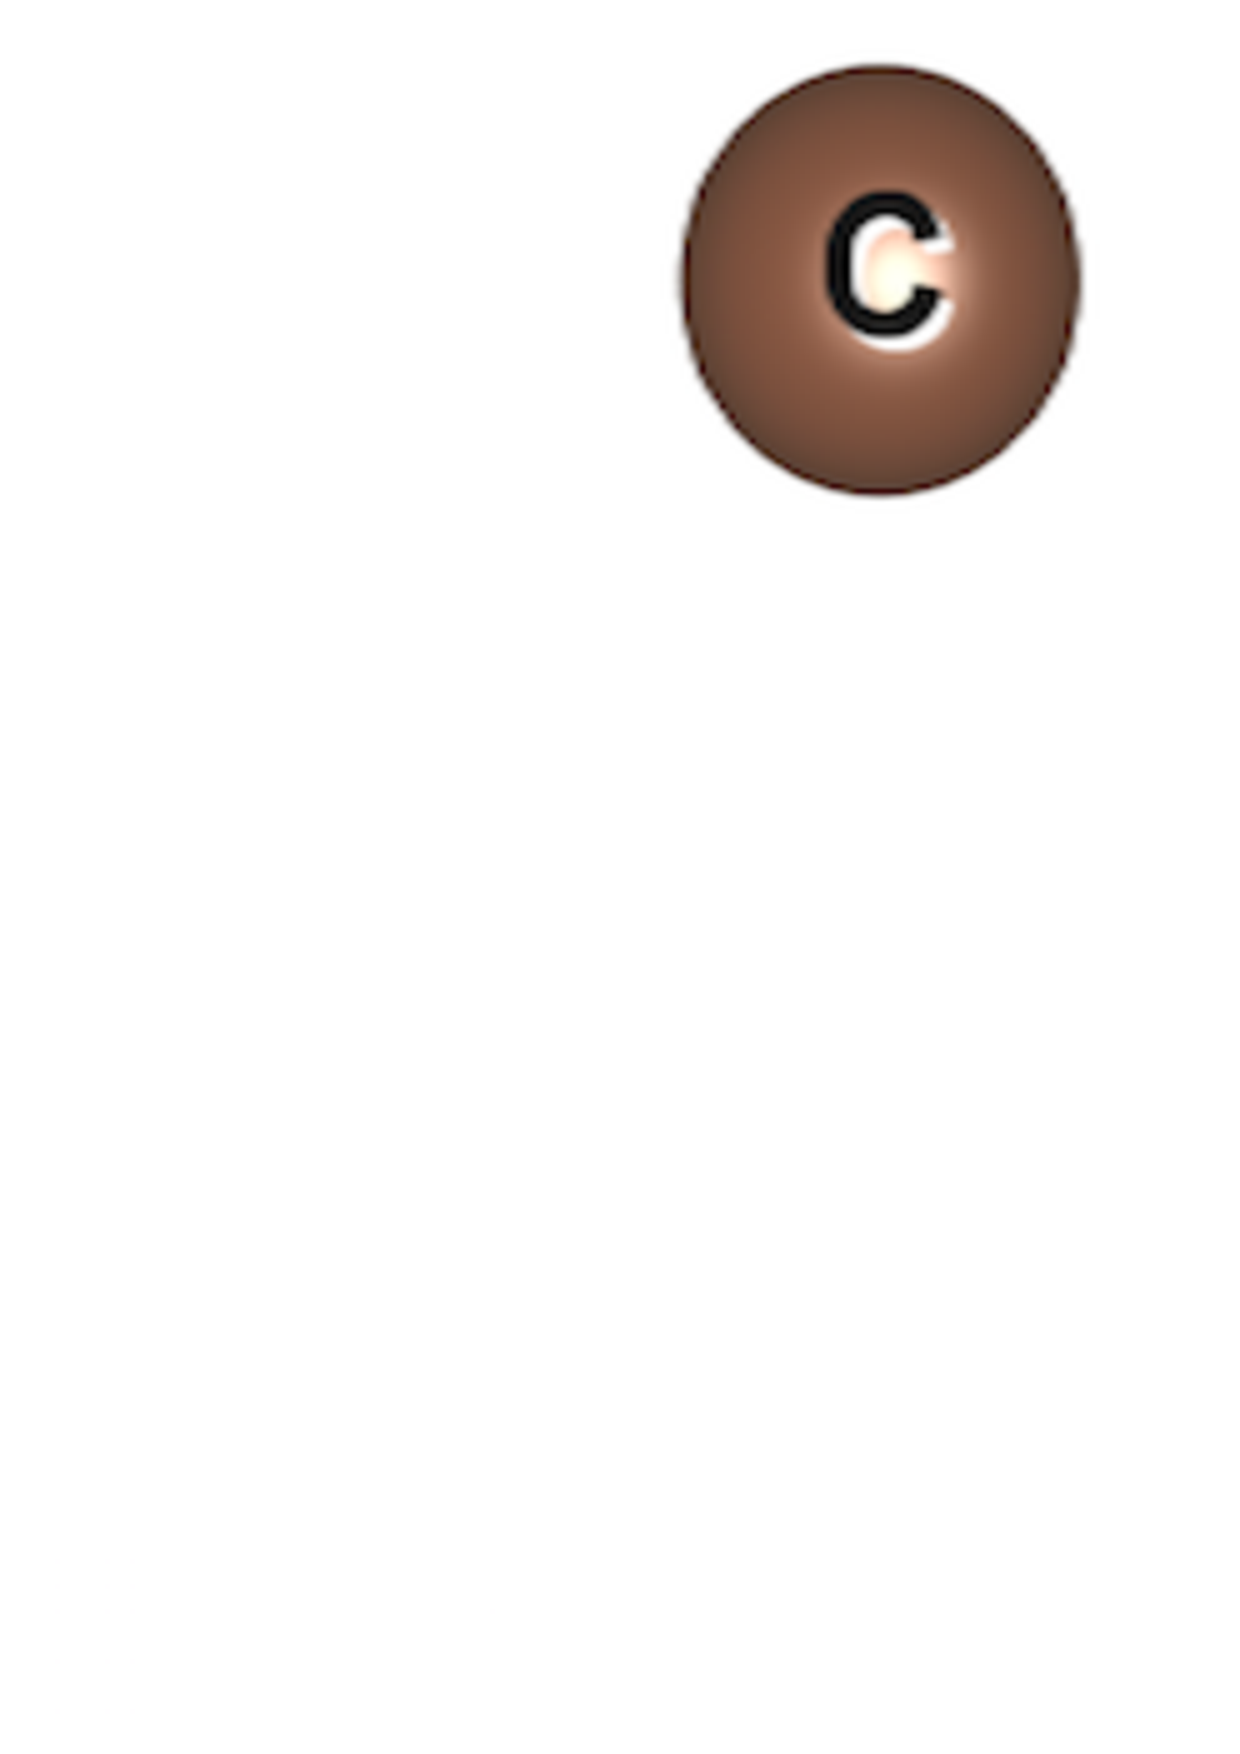
\includegraphics[clip, width=0.30\textwidth]{c_pi.png}}
    \subfigure[]{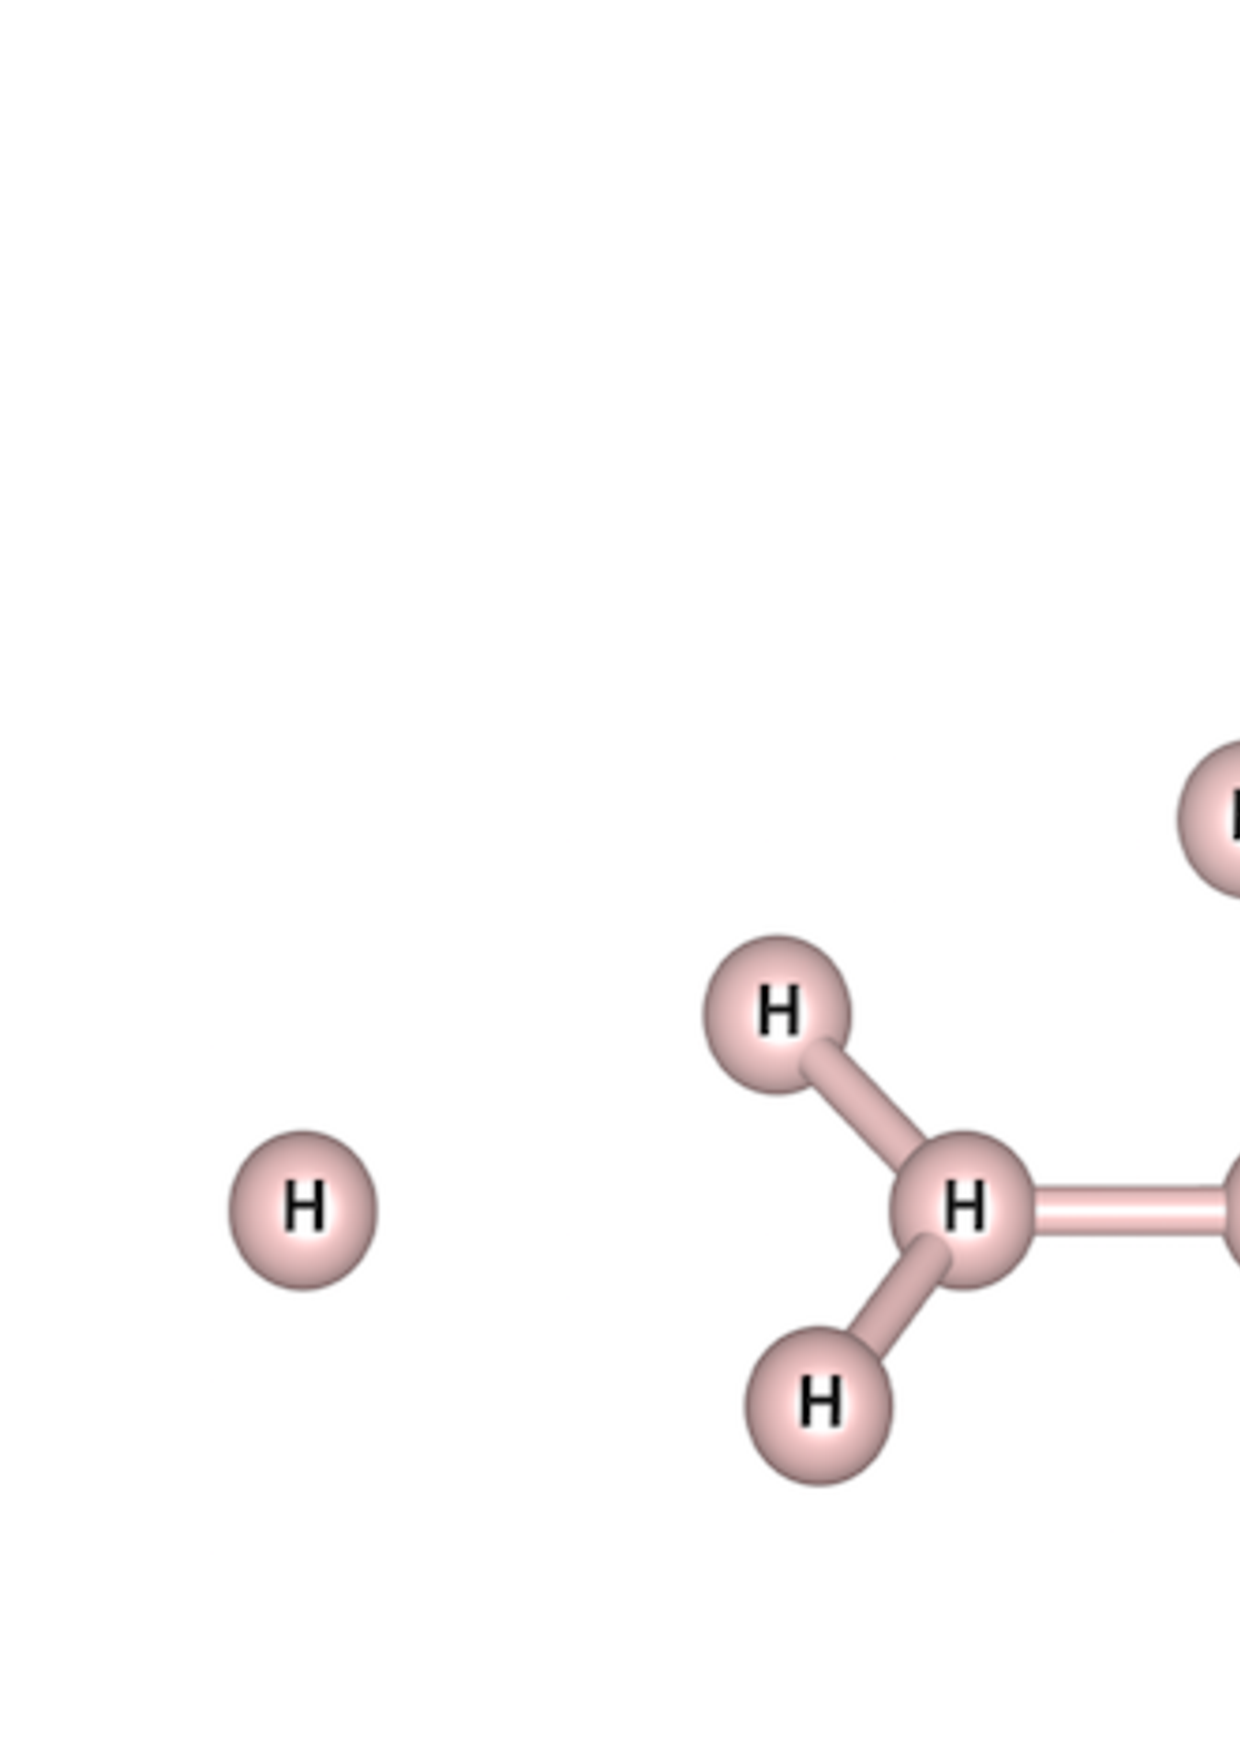
\includegraphics[clip, width=0.30\textwidth]{h_wan.png}}
       \caption{Wannier orbitals constructed from Kohn-Sham orbitals: (a) graphene $\sigma$ orbital; (b) graphene $\pi$ orbitals; (c) hydrogen S orbital. }
\label{fig:wan}
\end{figure*}

We choose a set of Slater-Jastrow wave functions corresponding to the electron-hole excitations within the $\pi$ channel. The energy expectation expressed in terms of the density matrices is, 
\begin{eqnarray}\label{eq:en}
E = C + t(\sum_{\langle i, j\rangle, \sigma} \rho_{ij}^\sigma + \rho_{ji}^\sigma) + U \sum_{i}M_{ii;ii}^{\uparrow,\downarrow}\,,
\end{eqnarray}
If we have n wave functions, we can form a linear least problem of $n\times 3$ from the n constraints of Eq.~\eqref{eq:en}.
\begin{eqnarray}
\begin{pmatrix}
E_1\\
E_2\\
\cdots\\
E_n
\end{pmatrix}=
\begin{pmatrix}
1 & \quad \Big[\sum_{\langle i, j\rangle} \rho_{ij}^\sigma + \rho_{ji}^\sigma\Big]_{1} & \quad \Big[\sum_{i}M_{ii;ii}^{\uparrow,\downarrow}\Big]_1\\
1 & \quad \Big[\sum_{\langle i, j\rangle} \rho_{ij}^\sigma + \rho_{ji}^\sigma\Big]_{2} & \quad 
\Big[\sum_{i}M_{ii;ii}^{\uparrow,\downarrow}\Big]_2\\
\cdots & \quad \cdots & \quad \cdots \\ 
1 & \quad \Big[\sum_{\langle i, j\rangle} \rho_{ij}^\sigma + \rho_{ji}^\sigma\Big]_{n} & \quad 
\Big[\sum_{i}M_{ii;ii}^{\uparrow,\downarrow}\Big]_n\\
\end{pmatrix}
\begin{pmatrix}
C\\
t\\
U
\end{pmatrix}\,.
\end{eqnarray}
Table~\ref{tab:grpheffm} shows the final results using 25 wave functions. The errorbar is calculated using Jackniff method.  
\begin{table}[ht]\caption{Downfolding parameters for graphene and hydrogen.}\label{tab:grpheffm}
\centering
\begin{tabular}{|c|c|c|}
\hline
parameters [eV] & graphene &hydrogen \\
\hline
\hline
t & 3.61(1) & 3.73(1)\\
U & 7.16(3) & 9.47(5)\\
\hline
\end{tabular}
\end{table} 
Fig.~\ref{fig:ne_aidmd_gh} shows fitted energies versus the \textit{ab initio} VMC energies. We find that the onsite Hubbard model describes graphene and hydrogen very well. The ratio of t/U is small than the semimetal-insulator transition critical value (3.8) in both the two systems, consistent to the fact that both the two systems are semimetals.  
\begin{figure}[htb]
\centering
\subfigure[]{\includegraphics[width=0.45\textwidth]{grp_all_tu.pdf}}
\subfigure[]{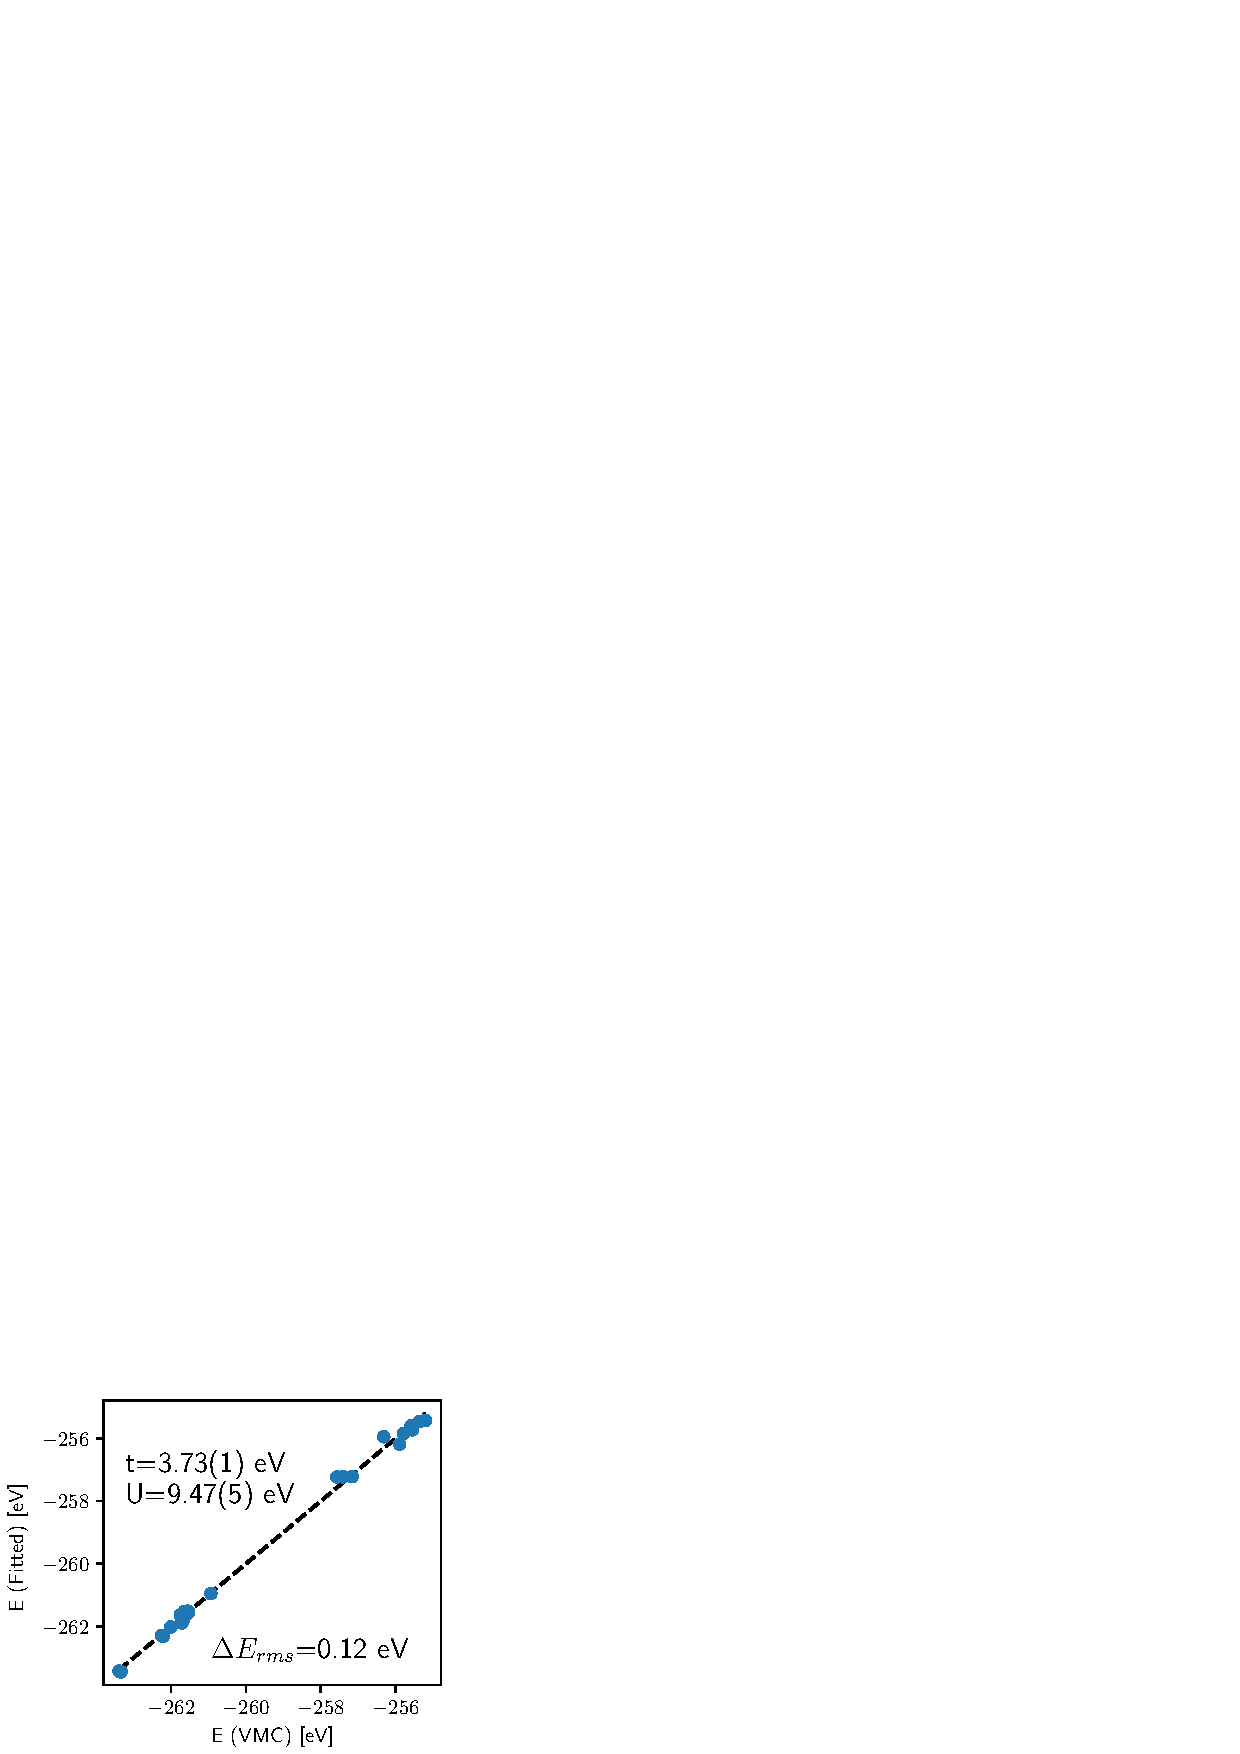
\includegraphics[width=0.45\textwidth]{h_tu.pdf}}
\caption{Comparison of \textit{ab initio} (x-axis) and fitted energies (y-axis) of the 3$\times$3 periodic unit cell of graphene and hydrogen lattice: (a) graphene; (b) hydrogen lattice.}\label{fig:ne_aidmd_gh}
\end{figure}

\section{Conclusion}
We have demonstrated three AIDMD methods where \textit{ab initio} QMC data are used to fit simple effective Hamiltonians. We have elaborated on the fitting procedures. The limitations of the model are judged by assessing the quality of the fitted energies and two-body density matrices or EKT matrix elements. This feature is useful for constructing refined models needed for the accurate simulation of real materials.

This approach can be used to identify important physics degrees of freedom in complex systems for understanding macroscopic phenomena. We are at the position of applying it to more complex systems, such as transition metal oxides, high Tc cuprates. 
%\include{tail}
\bibliographystyle{unsrt}
\bibliography{thesis}
\end{document}